%
% funktion.tex
%
% (c) 2018 Prof Dr Andreas Müller, Hochschule Rapperswil
%
\subsection{Funktion einer Kamera\label{subsection:kamerafunktion}}
Ziel dieses Abschnitts ist, eine Abstraktion einer Kamera zu finden,
welche sich einerseits geometrische einfach analysieren lässt aber
andererseits ein gutes Modell für eine genügend grosse Klasse von
real existierenden Kameras ist.
Komplizierter gebaute Kameras können dann wenn nötig durch Erweiterung dieses
Grundmodells beschrieben werden.
\subsubsection{Aufbau einer Kamera}
\begin{figure}
\centering
\includegraphics{applications/kamera/kamera.pdf}
\caption{Wichtigste Komponenten einer Kamera. Im roten Kameragehäuse befindet
sich der Bildsensor-Chip mit seiner Steuer- und Interface-Elektronik.
Das Bild wird vom Objektiv auf dem Chip erzeugt.
\label{applications:kamera:kamera-bild}}
\end{figure}
\begin{figure}
\centering
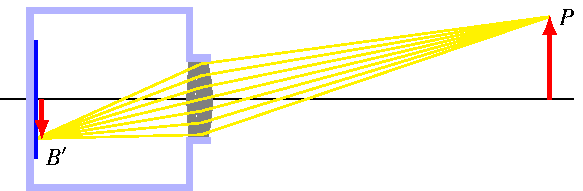
\includegraphics{applications/kamera/kameraprinzip.pdf}
\caption{Funktionsweise einer Kamera. Das Objektiv fokusiert den
Weltpunkt $P$ in den Bildpunkt $B$ auf dem Bildsensor ({\color{blue}blau}).
\label{applications:kamera:kameraprinzip}}
\end{figure}
Abbildung~\ref{applications:kamera:kamera-bild} zeigt die beiden in unserem
Zusammenhang wesentlichen Komponenten einer Kamera.
Das Objektiv fokusiert das von den abzubildenden Objekten ausgestrahlte
Licht und formt so ein Bild auf der Ebene des Bildsensors.
Eine Steuer- und Interface-Elektronik liest die Bilddaten aus dem Chip
aus, digitalisiert sie und macht sie zum Beispiel über ein USB-Interface
für einen Computer zugreifbar.
Einem Weltpunkt $P$ im dreidimensionalen Raum wird auf diese Weise ein
Bildpunkt $B$ auf der Chip-Ebene zugeordnet.

Die Qualität des erzeugten Bildes wird wesentlich bestimmt durch das
Objektiv.
Je grösser seine Öffnung ist, desto mehr Licht steht auf dem Chip zur
Verfügung.
Eine grosse Öffnung macht es aber auch schwierig, eine scharfe Abbildung
zu erreichen.
Die Lichtstrahlen am Rand einer grossen Linse werden nicht in den gleichen
Brennpunkt fokusiert wie die Strahlen, die die Linse Nahe dem Zentrum
passieren.
Mit einem einfachen zweilinsigen Objektiv wie in
Abbildung~\ref{applications:kamera:kamera-bild} ist das Bild nur nahe
der optischen Achse wirklich scharf.
Moderne Objekte verwenden daher mindestens vier oder noch mehr Linsen,
oder sogar Linsen, deren Oberfläche nicht sphärisch geschliffen ist.

\begin{figure}
\centering
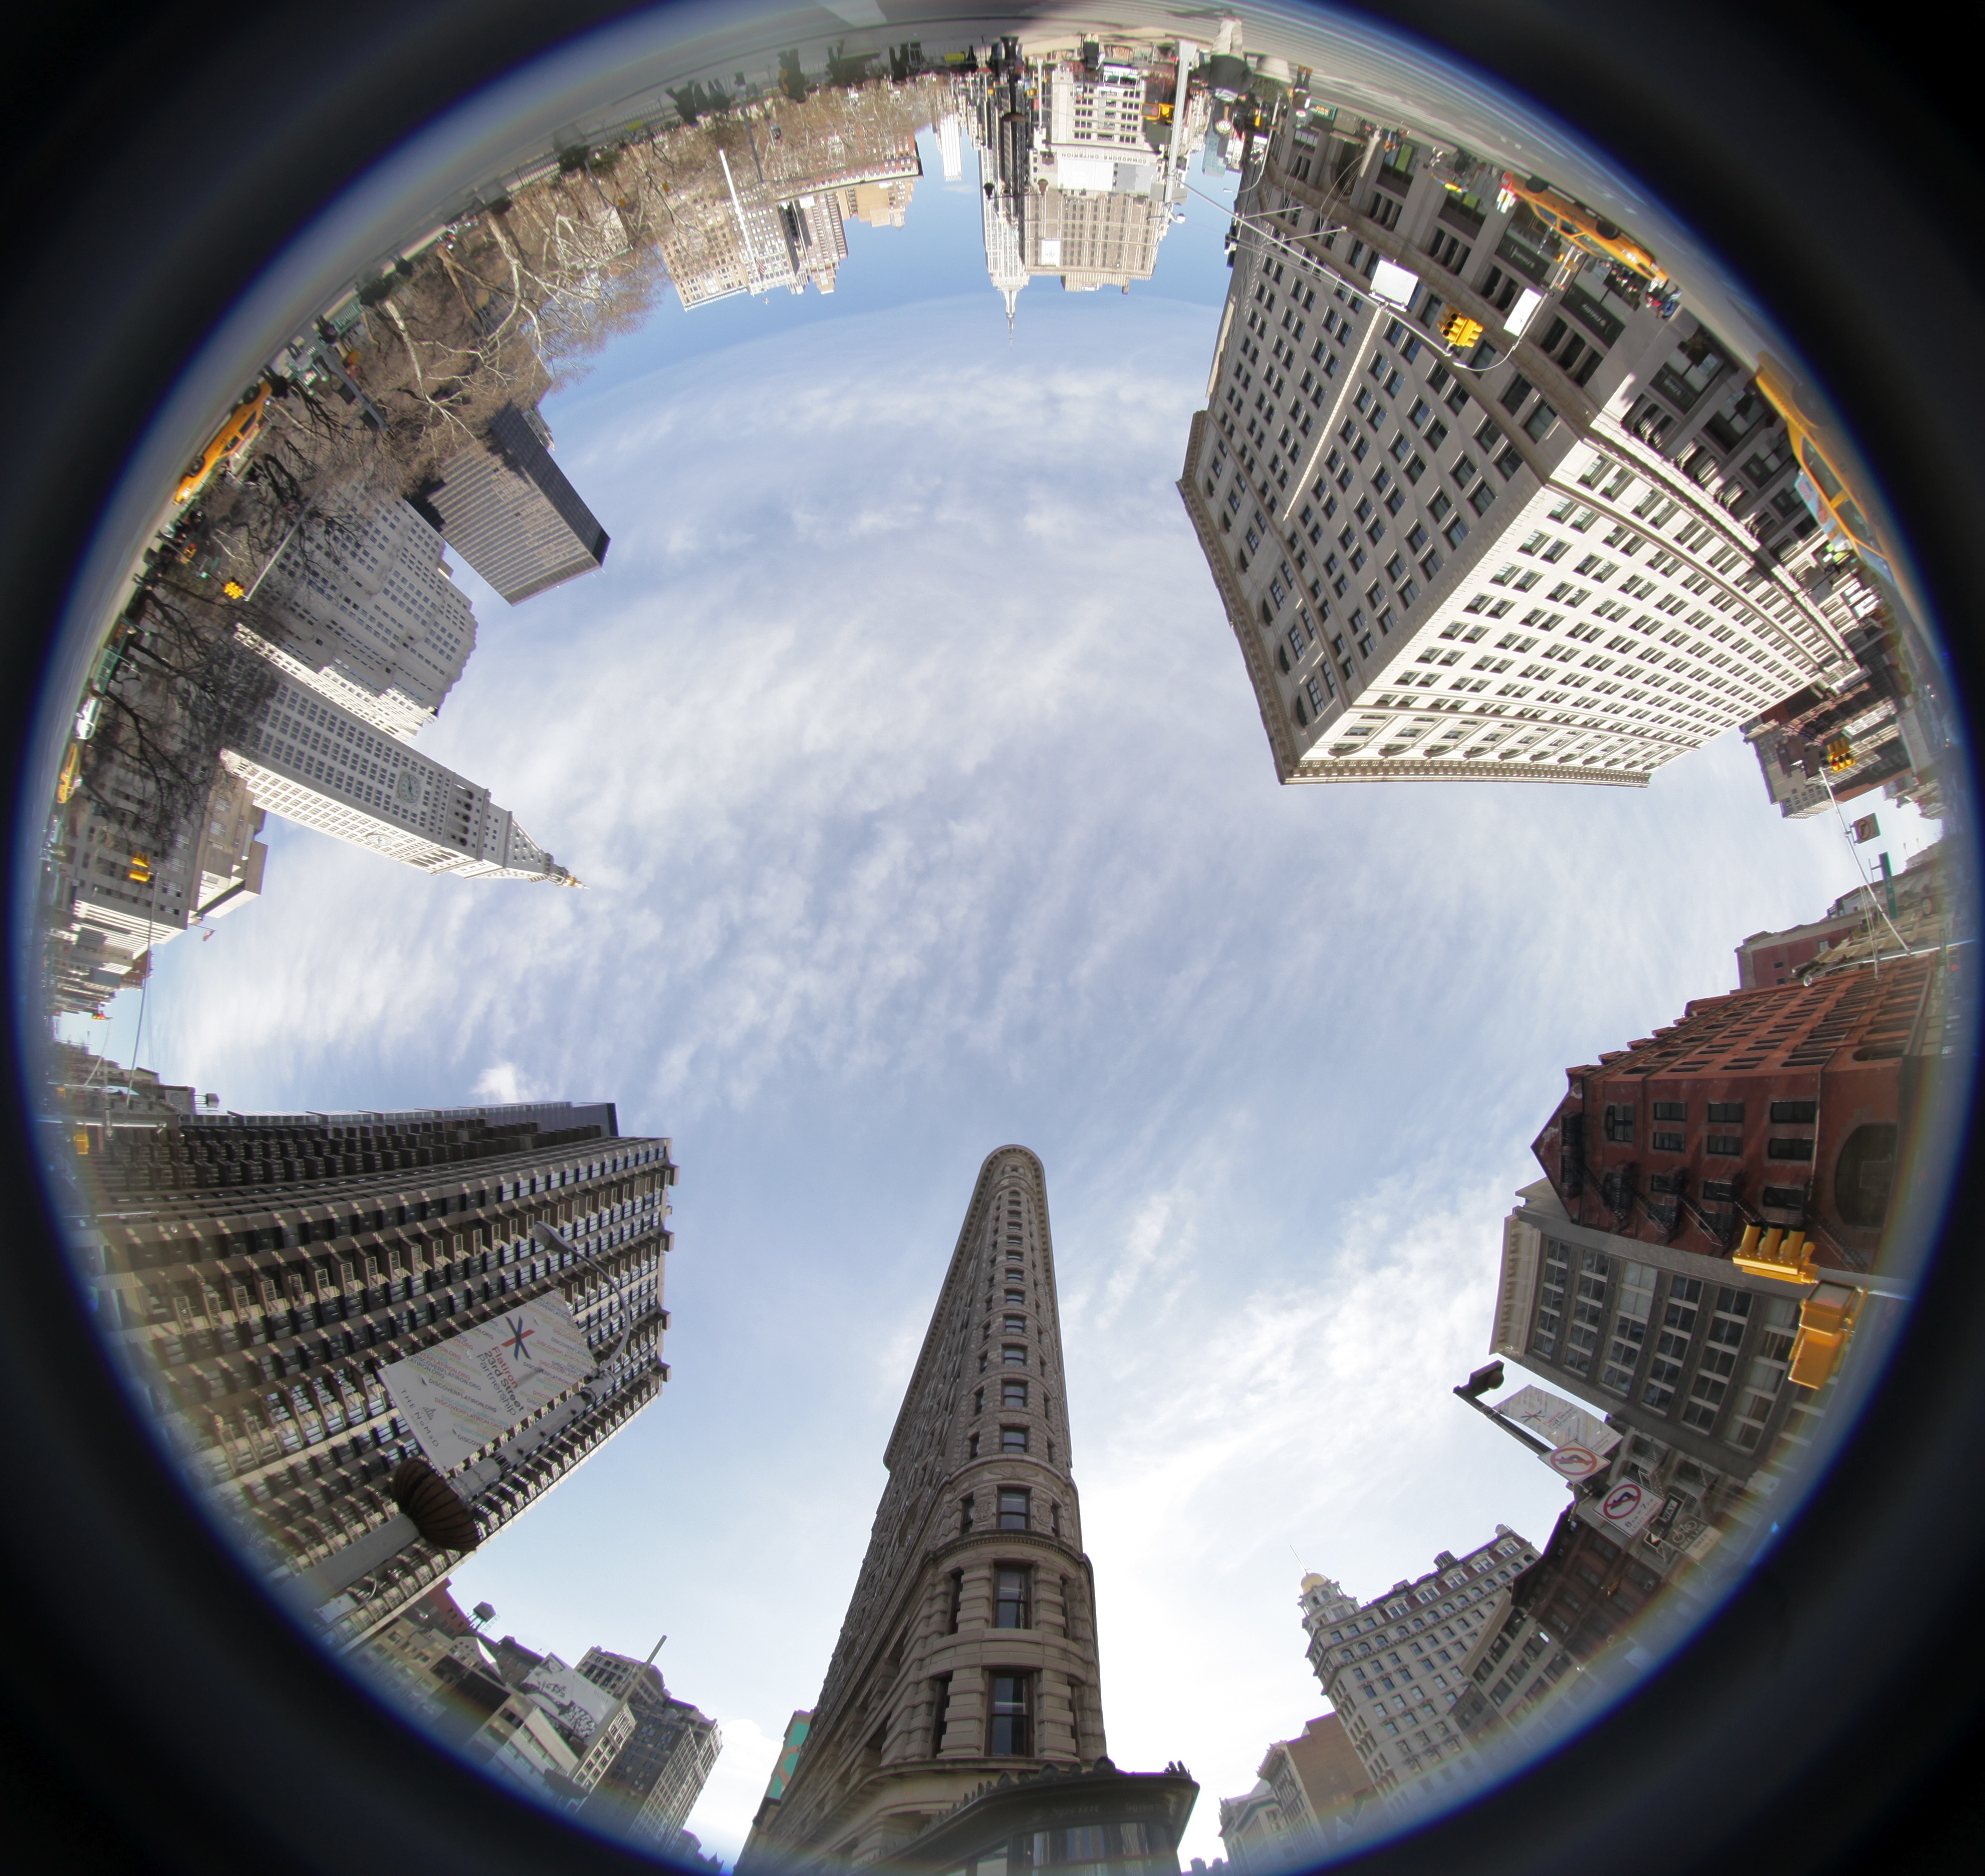
\includegraphics[width=8cm]{applications/kamera/fisheye.jpg}
\caption{Ein Fischauge-Objektiv bildet eine $180^\circ$-Gesichtsfeld in
einen Kreis ab.
Dabei werden Geraden in gekrümmte Linien abgebildet.
\label{applications:kamera:fisheye}}
\end{figure}%
Objektive sehr kurzer Brennweite können oft nicht ohne radiale Verzerrungen
gebaut werden.
Besonders ausgeprägt ist dies bei den Fischauge-Objektiven
(Abbildung~\ref{applications:kamera:fisheye}), die
ein Gesichtsfeld von $180^\circ$ in einen Kreis abbilden können.
Sie zeichnen sich dadurch aus, dass Geraden im Raum auf gekrümmte
Linien auf dem Bild abgebildet werden, solche Objektive lassen sich
also nicht mit einer linearen Abbildung beschreiben.

\subsubsection{Lochkamera}
Um die Analyse der Kameraabbildung zu vereinfachen stellen wir uns vor,
dass der Durchmesser des Objektivs immer kleiner gemaht wird.
Die Abbildungsfehler, die durch die Krümmung der Linse in den Randzonen
hervorgerufen wird, fallen dann weg.
Die Linse wirkt dann nur noch wie ein winzig kleines Loch, die Krümmung
der Linse ist nicht mehr von Bedeutung.
\begin{figure}
\centering
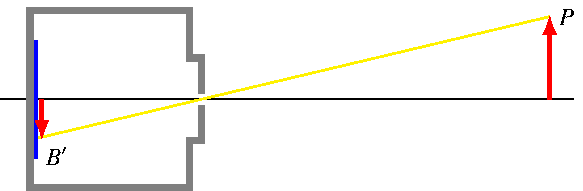
\includegraphics{applications/kamera/lochkamera.pdf}
\caption{Vereinfachung der Kamera von
Abbildung~\ref{applications:kamera:kameraprinzip} zu einer Lochkamera
\label{applications:kamera:lochkamera}}
\end{figure}
Eine solche Lochkamera ist ein vereinfachtes Modell für Kameras mit
nicht zu kurzer Brennweite.

Die Abbildung einer Lochkamera ist geometrisch sehr einfach.
Ein vom Weltpunkt $P$ ausgehender Lichtstrahl verläuft in gerader
Linie durch das Loch und schneidet die Chip-Ebene im Bildpunkt $B$.
Eine Gerade $g$ im Raum wird von einer Schar von Geraden durch das Loch und
die Geraden $g$ abgebildet.
Diese Geraden liegen alle in einer Ebene $\sigma$.
Die zugehörigen Bildpunkt liegen daher auf der Schnittgeraden der
Chip-Ebene mit der Ebene $\sigma$ der Abbildungsstrahlen.
Insbesondere bildet die Lochkamera Geraden immer wieder in Geraden ab.
Wir erwarten daher, dass diese Abbildung mit Hilfe von Matrizen
beschrieben werden kann.
